Im Punkt Fehlende im Menü "Data-Input" können fehlende Lehrer und fehlende Klassen eingegeben werden. Klickt man nun im Menü "Data-Input" (siehe \autoref{fig:instr_admin_absentees_dimenu}) auf Fehlende eintragen, dann gelangt man in ein weiteres Menü.(siehe \autoref{fig:instr_admin_absentees_menu}) In welchem man zwischen Klassen und Lehrer wählen kann. Wie der Name schon sagt, bei fehlende Lehrer werden die fehlenden Lehrer eingetragen und bei fehlenden Klassen werden die fehlenden Klassen eingetragen.
\begin{figure}[H]
\centering

\includegraphics[keepaspectratio=true, width=14cm]{images/screenshots/data-inputs2.png}
\caption{Data-Input-Menü}
\label{fig:instr_admin_absentees_dimenu}
\end{figure}
\begin{figure}[H]
\centering
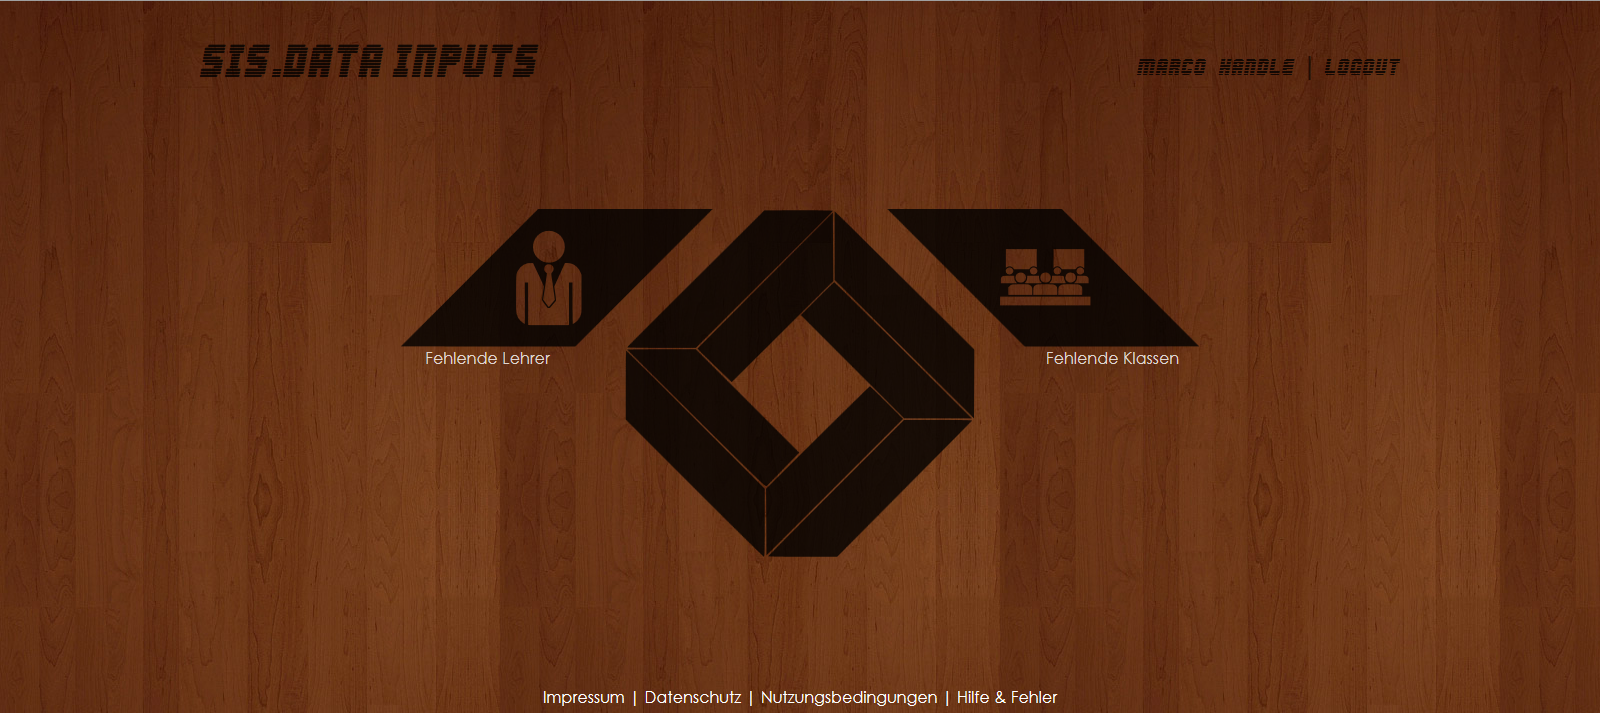
\includegraphics[keepaspectratio=true, width=14cm]{images/screenshots/data-inputs_absentees.png}
\caption{Fehlende Auswahl}
\label{fig:instr_admin_absentees_menu}
\end{figure}
\subsection{Fehlende Lehrer}
Hat man nun den Punkt fehlende Lehrer Ausgewählt, so gelangt man zur Eingabemaske, die wie in \autoref{fig:instr_admin_absentees_Lehrer} aufgebaut ist.
\paragraph{Hinzufügen}
Unter der Überschrift ist eine Auswahlmöglichkeit für das Datum, dieses Datum spiegelt den ersten Tag des Fehlens eines Lehrers wieder. Will man nun einen Lehrer als fehlend eintragen, so muss zuerst das Start-Datum gewählt werden. Dies kann entweder durch drücken der Pfeiltaste geschehen oder durch Eingabe des Datums in dem Textfeld zwischen den Pfeilen. Wird diese Möglichkeit genutzt, muss darauf geachtet werden, dass das Datum im Format yyyy-mm-dd eingegeben wird. Mit Enter muss diese Eingabe bestätigt werden.\\
Hat man nun das gewünschte Datum erreicht, so kann mit der Eingabe begonnen werden. Im ersten Feld, das mit Lehrer Beschriftet ist, muss das Lehrer-Kürzel eingetragen werden. Wird ein Buchstabe eingegeben so erscheint eine Liste von Lehrern, die diesen Buchstaben enthalten. Nachdem der Lehrer eingegeben wurde, muss die Start-Stunde eingegeben werden. Das Feld Starttag kann nicht verändert werden, dies entspricht immer dem oben eingestellten Datum. Als Start-Stunde sind die Werte 1-16 erlaubt, es sei denn es wurden in der Eingabe der Stunden etwas anderes definiert. (Eingabe Stunde siehe \autoref{sec:instr_other_hours}) Für den Endtag ist standardmäßig auch das Start-Datum eingetragen, dieses kann jedoch in das gewünschte Datum geändert werden. Voraussetzung dafür ist, dass es größer oder gleich dem Startdatum ist und es muss im Format yyyy-mm-dd eingegeben werden. Außerdem muss beachtet werden, dass dieses Datum kein Wochenende sein darf. Also es muss ein Datum eingegeben werden, welches einem Wochentag zwischen Montag und Freitag entspricht. Im letzten Feld kann  ein Grund für das Fehlen eingetragen werden. Ist alles wie gewünscht ausgefüllt, (Bis auf den Grund müssen alle Felder ausgefüllt werden) so kann auf Übernehmen geklickt werden.\\
Wird ein Lehrer oder eine Stunde nicht gefunden, so wird ein Pop-Up angezeigt, auf dem der Name der falschen Textbox steht, der beispielsweise, wie in \autoref{fig:instr_admin_absentees_fail} zu sehen ist, aussehen kann. Dieser muss mit OK bestätigt werden. Anschließend muss die Eingabe erneut erfolgen.\
\subsection{Verändern}
Soll ein vorhandener Eintrag verändert werden, so kann das auf einfache weise gemacht werden. Dabei kann einfach der Eintrag verändert werden. Ist alles nach den neuen Wünschen angepasst, so muss auf Übernehmen geklickt werden, um den Eintrag zu übernehmen.
\subsection{Löschen}
Ist ein Eintrag fehlerhaft oder muss er entfernt werden, so muss ein Hacken bei Löschen, in der Zeile des zu löschenden Eintrages, gesetzt werden und anschließend mit übernehmen bestätigen. (siehe \autoref{fig:instr_admin_absentees_Leherer_delete}) Nun ist dieser Eintrag \textbf{unwiderruflich} gelöscht.
\begin{figure}[H]
\centering
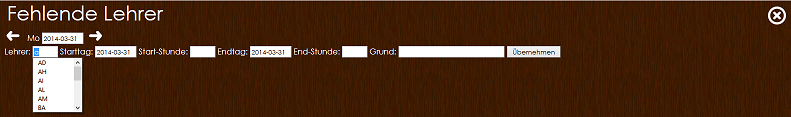
\includegraphics[keepaspectratio=true, width=16cm]{images/screenshots/absentees_teacher.png}
\caption{Fehlende Lehrer}
\label{fig:instr_admin_absentees_Lehrer}
\end{figure}
\begin{figure}[H]
\centering

\includegraphics[keepaspectratio=true, width=4cm]{images/screenshots/input_fail_teacher.png}
\caption{Falsche Eingabe}
\label{fig:instr_admin_absentees_fail}
\end{figure}
\begin{figure}[H]
\centering

\includegraphics[keepaspectratio=true, width=16cm]{images/screenshots/absentees_teacher_delete.png}
\caption{Fehlenden Lehrer löschen}
\label{fig:instr_admin_absentees_Leherer_delete}
\end{figure}
\subsection{Fehlende Schüler}
Die Eingabe der Fehleden Schüler läuft exakt nach dem gleichen Verfahren und Regeln ab wie die Eingabe der Fehlenden Lehrer. Deshalb werde ich hier nichts mehr zur Eingabe der fehlenden Klassen schreiben.